\chapter{Počítačové vidění v endoskopii}
\section{Úvod do počítačového vidění}
Počítačové vidění (dále jen \gls{glos:CV}) je obor výpočetní techniky jehož počátky sahají do 60. let minulého století. Tomuto oboru se v posledních letech dostalo velkého rozmachu. Na trh se dostává stále více zařízení schopných snímat obrazová data,vzrůstá jejich kvalita a cena klesá. Ač \gls{glos:CV} není vyloženě určeno nějakou definicí,dalo by se říci, že \gls{glos:CV} je strojové porozumění obrazu, který se získává ze snímacích zařízení (např. různé fotoaparáty či kamery). V podstatě by se dalo srovnat s viděním biologickým s tím rozdílem, že u většiny vícebuněčných organismů jde o naprosto přirozenou a běžnou věc.\cite{learning}\cite{image} \gls{glos:CV} najde zastoupení v celé řadě odvětví např.

\begin{itemize}
	\item Automatizovaný průmysl - čidla pro kontrolu vadností výrobku, ovládání robotů, řízení logistických procesů, ...
	\item Medicína - zpracování obrazových dat z mikroskopů, ultrazvuku, endoskopii, RTG, ... \gls{glos:CV} zkvalitňuje diagnostické nástroje a je již standardní součástí diagnostických procesů.
	\item Armáda - automaticky naváděné rakety, detekce pohybu vojáků, bezpilotní stroje (letadla, ponorky, ...)
	\item Zábavní průmysl - interakce mezi strojem a člověkem. Např. ovládání počítačové hry gesty.
	\item Rozšířená realita - v kombinaci s počítačovou grafikou je základním prvkem v rozšířené realitě. Např. Microsoft hololens.
	\item A mnoho dalších.
\end{itemize}

Oproti biologickému vidění se jedná z pohledu zpracování o velice komplikovanou věc. Počítač přijímá pouze číselné hodnoty jako obrazová data. Proto je pro lidský druh snadné identifikovat např. auto na obrázku \ref{fig:car}, ale pro stroj je nutné definovat auto, jako složitý matematický model. \gls{glos:CV} také naráží na problémy, které vznikají při sběru dat. Jsou jimi: (volně přeloženo z \cite{image}).
\begin{itemize}
	\item 3D > 2D - ztráta prostorové informace. Obraz z reálného světa je uložen jako 2D. Díky modelu dírkové komory\footnote{z anglického pinhole model} jsou malé objekty blízké kameře stejné jako velké vzdálené objekty. Lidé jsou schopni tyto objekty rozeznat, pokud je v obraze nějaký objekt, u kterého znají jeho velikost, např. krabička od sirek.
	\item Interpretace - porozumění obsahu scény. Lidský mozek vyhodnocuje obraz pomocí svých znalostí a zkušeností. A proto je schopný vyhodnocovat nové problémy, které předtím neznal. Zatímco takováto schopnost strojů je velice omezená a její zdokonalení je klíčem k inteligentním systémům. Počítač je schopen analyzovat obraz pomocí matematické logiky, sémantiky a teorií formálních jazyků. Pokud je znám algoritmus pro řešení určitého problému, je možno analyzovat obraz, např. řeka v satelitním obrazu.
	\item Šum - je přítomný v každém měření v reálném světě.
	\item Příliš mnoho dat - Obrázky a videa jsou obrovské. Stránka A4, 300 dpi, 8 bit per pixel = 8,5 MB. Neprokládané video 512 x 768, RGB (24 bit) = 225 MB/s. Je proto tak těžké dosáhnout složité analýzy v reálném čase.
	\item Měřený jas - je dán složitým fyzikálním postupem vytváření obrazu. Zář závisí na ozáření (typ světelných zdrojů, jejich poloha a intenzita),
	poloze pozorovatele, lokální geometrii povrchu a odrazivosti povrchu.
	Obrácená úloha je špatně podmíněna.
	\item Lokální okno versus potřeba globálního pohledu - počítač vidí svět pouze z pohledu klíčové dírky bez celkového kontextu. Je proto těžké určit kontext obrazu, pokud je dostupná jen jeho část. Lidský mozek je schopný si domyslet potřebné informace pro určení, pokud je zná.
\end{itemize}

\begin{figure}[h]
	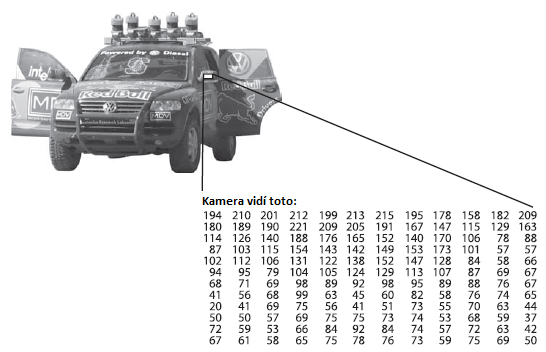
\includegraphics[]{car}
	\centering
	\caption{Auto přeloženo z\cite{learning}\label{fig:car}}
\end{figure} 


Zpracování obrazu počítačem se dá rozdělit na několik úrovní a výsledkem je řetězec, kde se postupuje od nejnižší po nejvyšší úroveň. Na nejnižší úrovni se zpracovávají surová data, která jdou přímo ze snímacích senzorů. Poté, co je obraz z nejnižší úrovně zpracován, používají se metody pro odstranění šumu, detekce hran, barevná filtrace či různá komprese obrazu. Těmito úpravami vznikne obraz, ze kterého lze již přejít k vyšší úrovni zpracování a tím je porozumění daného obrazu. Na této úrovni se dají aplikovat poznatky z umělé inteligence (např. neuronové sítě) nebo matematické definování objektů pro určení výsledného významu obrazu. Vyšší úroveň zpracování je nejtěžší věc na \gls{glos:CV}, často není ani možné dosáhnout požadovaného výsledku a vše se musí zjednodušovat, aby se dosáhlo alespoň výsledku částečného. \cite{learning}\cite{image}

\section{Algoritmy počítačového vidění}
V biomedicíně se používá většina známých algoritmů z počítačového vidění. Jelikož je jich velké množství, jsou pro charakter této práce popsány pouze ty, které se pak používají v praktickém řešení konkrétního problému této práce. Všechny tyto základní známé algoritmy jsou implementovány v knihovnách či programech pro počítačové vidění, např. OpenCV nebo Matlab.

\subsection{Konverze barevných formátů}
Obrazová data, s nimiž se v počítačovém vidění pracuje, jsou reprezentována různými grafickými schématy. V této práci se vyskytuje převážně schéma RGB, ve kterém jsou uložena data. Dále se pracuje s HSV a GrayScale.

\begin{itemize}
	\item RGB formát je aditivní míchání červené, zelené a modré barvy. Každý bod na obrázku je udáván jako vektor tří elementů, tedy intenzitou tří základních barev.\cite{image}
	\item HSV formát se skládá ze tří složek: barevný tón(hue), sytost(saturation) a hodnota jasu neboli množství bílého světla (value). Je velice blízký lidskému vnímání barvy a to zejména tónu a sytosti. Tento formát se hojně používá při algoritmech pracujících s obrazem.\cite{image}
	\item Grayscale vyjadřuje data pouze v odstínech šedi. Každá hodnota je definována na stupnici šedi a výsledný obraz je tak černo-bílý.
\end{itemize}

Převody mezi těmito formáty nejsou triviální záležitostí a jsou pro ně definovány složité vzorce. Na obrázku \ref{fig:colorspace} lze vidět ukázku barevných schémat. 

\begin{figure}[h]
	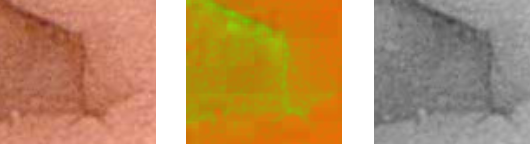
\includegraphics[scale=0.5]{colorspace}
	\centering
	\caption{Barevná schémata zleva: RGB, HSV a GrayScale}\label{fig:colorspace}
\end{figure}

\subsection{Práhování}
Práhování\footnote{Z anglického threshold} je nejjednodušší z metod segmentace obrazu. Metoda spočívá v definování hranice hodnot, která bude sloužit pro rozhodnutí, bude-li daný bod v obraze  akceptován či nikoliv. To, co se bude dít s akceptovaným a neakceptovaným bodem, záleží na konkrétní metodě. Mezi základní patří:\cite{opencv}

\begin{itemize}
	\item Binární - Akceptovaný bod je nastaven na 1, ostatní na 0.
	\item Osekání - Akceptovaný bod je ponechán. Ostatní jsou zahozeny.
	\item Do nuly - Pokud je bod menší než daná hranice, tak je nastaven na 0. Ostatní jsou ponechány.
\end{itemize}

\begin{figure}[h]
	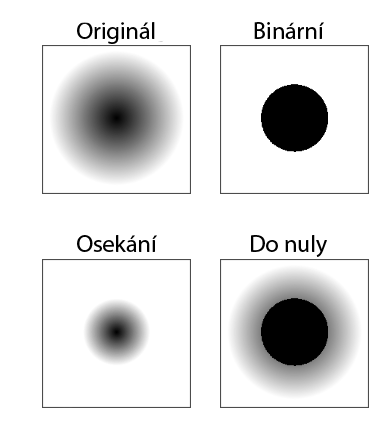
\includegraphics[scale=0.5]{threshold}
	\centering
	\caption{Metody práhování převzato z \cite{opencv}}\label{fig:threshold}
\end{figure}

Mezi složitější metody práhování patří adaptivní práhování, kde práh není stejný po celou dobu běhu algoritmu, ale je určován dynamicky. Dá se tím docílit lepších výsledků  při různých světelných podmínkách. Hodnota práhu může být vypočítána průměrem okolních hodnot nebo pomocí váženého součtu okolních bodů, kde váhy jsou Gaussovo okno.\cite{opencv}

\subsection{Morfologické operace}
Morfologické operace představují zpracování snímků založených na tvarech. Ve struktuře se generuje vstupní obraz na výstupní obraz. Uplatnění nachází především v oblastech spojování nesourodých prvků v obraze, hledání intenzity hrbolů nebo dírek v obraze či změny tvaru a velikosti geometrických objektů. Mezi základní morfologické operace patří eroze a dilatace.\cite{eroding}

Dilatace se skládá z obrazu (A), který v sobě skrývá jádro (B) určitého tvaru, nejčastěji čtverce nebo kruhu. Jádro má definován tzv. kotevní bod, který představuje střed jádra. Toto jádro je skenováno přes obraz. Počítáním maximální hodnoty pixelu překrytého jádra B a obrazového pixelu v bodě poloze kotvy způsobí světlé oblasti v obraze.  Dilataci můžeme vyjádřit jako sjednocení posunutých bodových množin. Uplatní se především v případech nutnosti zaplnění malých děr, úzkých zálivů, zvětšení objektů či použití jako stavební kámen složitějších operací. \cite{eroding}

Eroze je považována za sestru dilatace. Umožňuje spočítání lokálního minima přes oblast jádra. Jádro B je skenováno přes obraz a výpočtem minimální hodnoty vrátí obrazový pixel kotevního bodu.\cite{eroding}

\begin{figure}[h]
	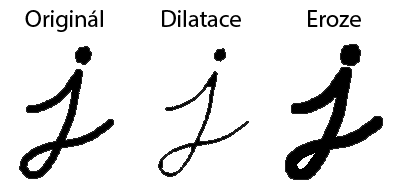
\includegraphics[scale=0.5]{morfoperace}
	\centering
	\caption{Morfologické operace převzato z \cite{eroding}}\label{fig:morfoperace}
\end{figure}

\subsection{Vyhlazování obrazu}
Vyhlazování obrazu, mnohdy také nazývané jako rozmazávání, je často používaná a jednoduchá operace při zpracování obrazu. Díky této operaci dosáhneme vyhlazení obrazu, například za účelem snížení šumu. Pro vyhlazování jsou používány nízkoprůchodové, nejčastěji lineární filtry, jako konvoluční matice. Tím se odstraní vysokofrekvenční obsah, např. hrany nebo šum.\cite{opencv:} Nejpoužívanější filtry jsou:

\begin{itemize}
	\item Normalizovaný filtr - pro každý pixel je spočítán průměr z jeho samého a okolí. Velikost okolí závisí na zvolené velikosti konvoluční matice. Filtr se používá pro odstranění vysokých frekvencí v obraze.\cite{opencv:}
	\item Gaussův filtr - konvoluční matice je vypočtena pomocí 2D Gaussovy rovnice. Jelikož by byl výsledek nekonečný, musí se specifikovat velikost matice a do ní se pak spočtou váhy Gaussova vrcholu. Filtr se používá pro odstranění šumu a vyhlazení obrazu.\cite{opencv:}
	\item Medián filtr - algoritmus vezme všechny pixely z konvoluční matice a určí jejich medián. Jím je pak nahrazen zpracovávaný pixel. Filtr se využívá pro odstranění "sůl a pepř" šumu.\cite{opencv:}
	\item Bilaterální filtr - je podobný Gaussovu filtru, ten bere v potaz všechny body, které se nachází v konvoluční matici, ale již neřeší jejich intenzitu. Bilaterální filtr proto používá ještě další funkci a zahrnuje pouze ty body v matici, jejichž intensita je podobná, jako právě zpracovávaného. To má za následek, že filtr vyhlazuje obraz, ale zachovává hrany. \cite{opencv:}
\end{itemize}

\begin{figure}[h]
	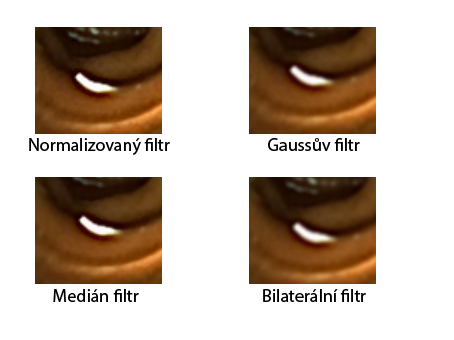
\includegraphics[scale=0.7]{filtry}
	\centering
	\caption{Ukázka filtrů z průběhu práce}\label{fig:filtry}
\end{figure}

\subsection{Detektory hran}
Detektory hran jsou velmi důležité pro algoritmy počítačového vidění. Neurofyziologický a psychofyzický výzkum ukazuje, že pro zrakové vnímání vyšších organismů jsou důležitá místa v obraze, kde se náhle mění hodnota jasu. Místa jež odpovídají významným hranám, nesou více informací než jiná místa v obraze. Je zde proto možné značně zredukovat množství dat, aniž by došlo k významné redukci informací o obraze.\cite{image}

Mezi nejpoužívanější hranové detektory patří Cannyho hranový detektor, který také završil hledání po ideálním detektoru hran. Byl vymyšlen Johnem F. Cannym v roce 1986 a míří k uspokojení tří kriterií:
\begin{itemize}
	\item Minimální počet chyb - algoritmus musí detekovat všechny důležité hrany a neměly by být detekovány žádné falešné výsledky.
	\item Přesnost - rozdíl polohy skutečné a detekované hrany musí být minimální.
	\item Jednoznačnost - pouze jeden výsledek pro jednu hranu. Toto je částečně pokryto bodem jedna - pro jednu hranu nelze detekovat více hran, ostatní by měly být falešné.
\end{itemize}

Cannyho algoritmus je se skládá z následujících kroků:
\begin{enumerate}
	\item Filtrování šumu obrazu pomocí Gaussovského filtru.
	\item Zjištění intensity gradientu pomocí Sobelova operátoru - aplikace konvolučních matic
	\item Potlačení bodů, které nejsou lokální maxima vzhledem ke směru gradientu. Tímto krokem se odeberou body, které nejsou považované za hranu. Pouze slabé linie zůstanou.
	\item Práhování s hysterezí zajistí výběr pouze významných hran. Určí se horní a dolní hranice práhování a hrany jsou pak vybrány na základě následujících pravidel:
	\begin{itemize}
		\item Pokud je hodnota gradientu větší než horní hraníce, pak je pixel přijat jako hrana.
		\item Pokud je hodnota gradientu menší než horní hraníce, pak je pixel odmítnut.
		\item Pokud je hodnota gradientu mezi hranicemi, je pixel přijat jen tehdy, je-li spojen s jiným pixelem, jehož hodnota gradientu je větší než-li horní hranice.
	\end{itemize}
\end{enumerate}

\begin{figure}[h]
	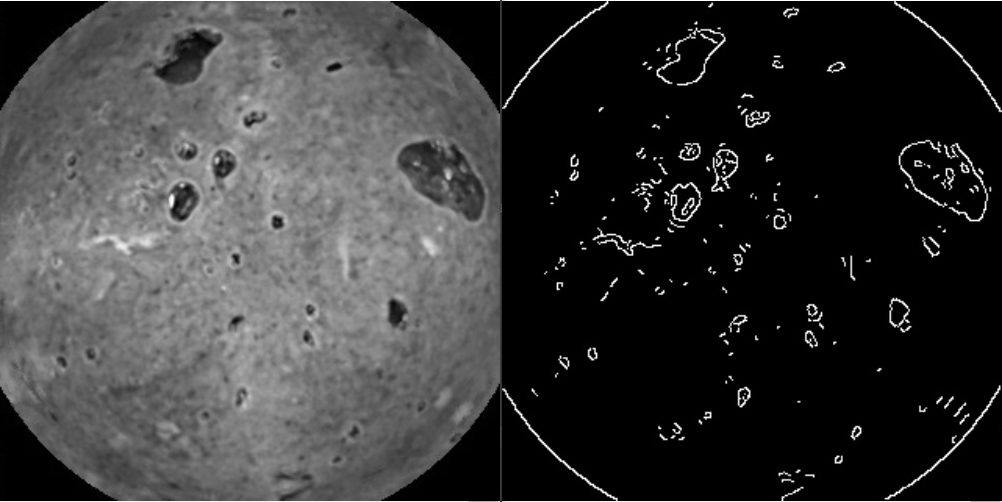
\includegraphics[scale=0.5]{cannyedge}
	\centering
	\caption{Ukázka Cannyho detektoru z průběhu práce}\label{fig:cannyedge}
\end{figure}


\section{Aktuální stav trhu}
\subsection{Rapid Software v8}
Rapid Software v8 je vyvinut společností Given Imaging, která mimo jíné vyrábí i kamery PillCam SB3. Jejich software je proto dodáván s těmito kamerami. Software umí spoustu užitečných věcí, ale pro charakter této práce je pouze podstatné, že nabízí detekci krve ve střevech. Škoda, že výrobce již neudává s jakou přesností. Na obrázku \ref{fig:rapid} je vidět ukázka rozhraní.\cite{pillcam}

\begin{figure}[h]
	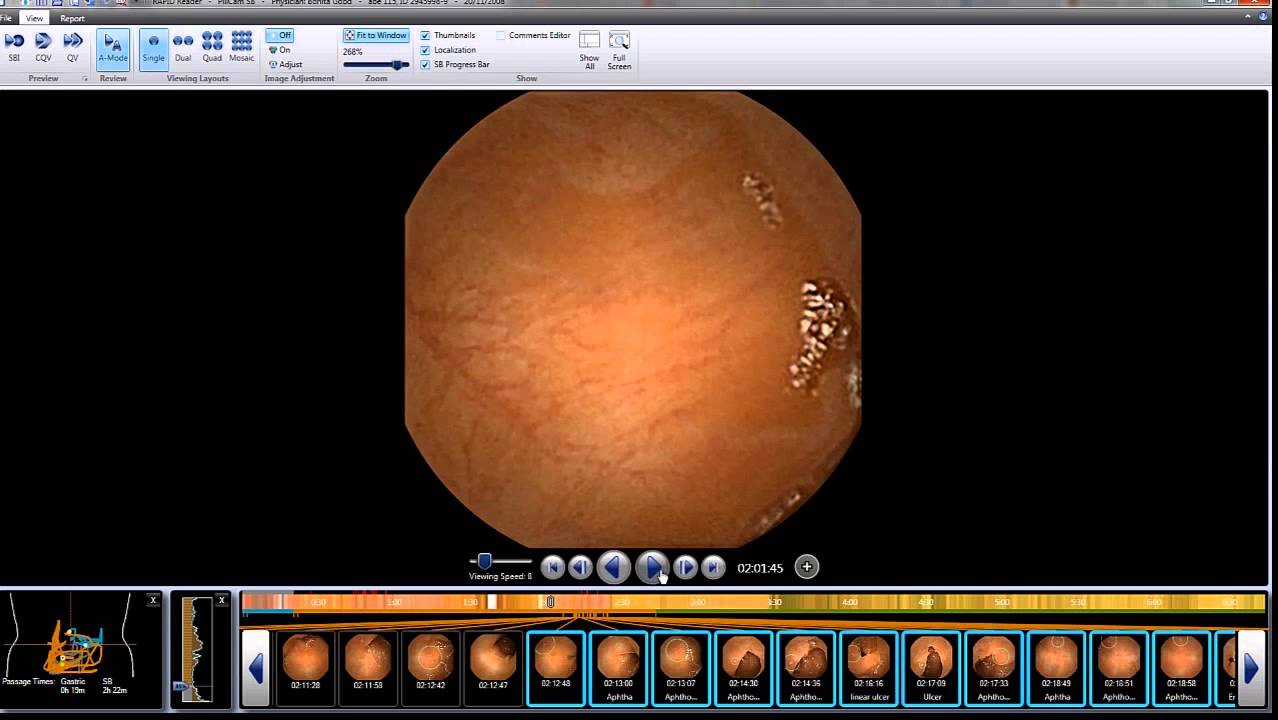
\includegraphics[scale=0.25]{rapid}
	\centering
	\caption{Ukázka Rapid v8\cite{rapidsoftware}\label{fig:rapid}}
\end{figure} 
\FloatBarrier

\subsection{Endocapsule 10 System}
Endocapsule 10 System je software vyvinutý společností Olympus, který ho také dodává ke svým kamerám. Software mimo základních věcí má algoritmy pro detekci červené barvy, bublin, nečistot a stejných obrázků. Díky těmto algoritmům je možné odfiltrovat nezajímavé či nehodnotné obrázky a nemusí se tak procházet celý vzorek. Ukázka rozhraní je vidět na obrázku \ref{fig:olympus}.\cite{endocapsule}

\begin{figure}[h]
	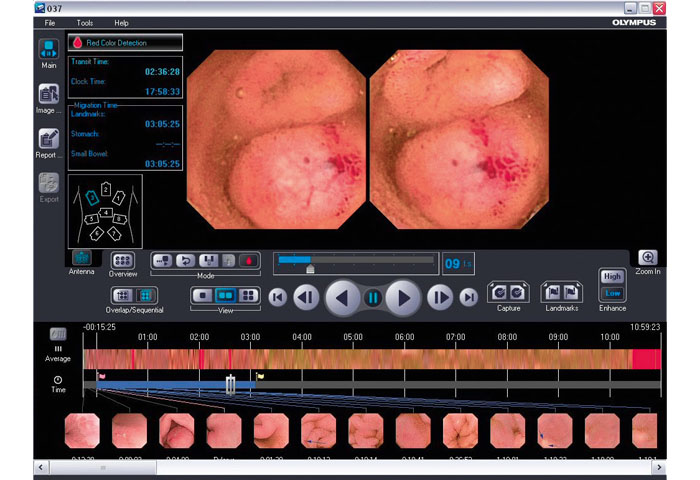
\includegraphics[scale=0.5]{olympus}
	\centering
	\caption{Ukázka Endocapsule 10 System \cite{olympuseuropa}\label{fig:olympus}}
\end{figure}
\FloatBarrier

\subsection{MiroView 2.5}
MiroView 2.5 je software vyvinutý společností IntroMedic, která taktéž dodává řešení se svými kamerami. Poskytuje základní funkcionalitu práce s videem a nabízí také automatickou detekci krve. Na obrázku \ref{fig:miroview} je vidět ukázka rozhraní.\cite{intromedic}

\begin{figure}[!h]
	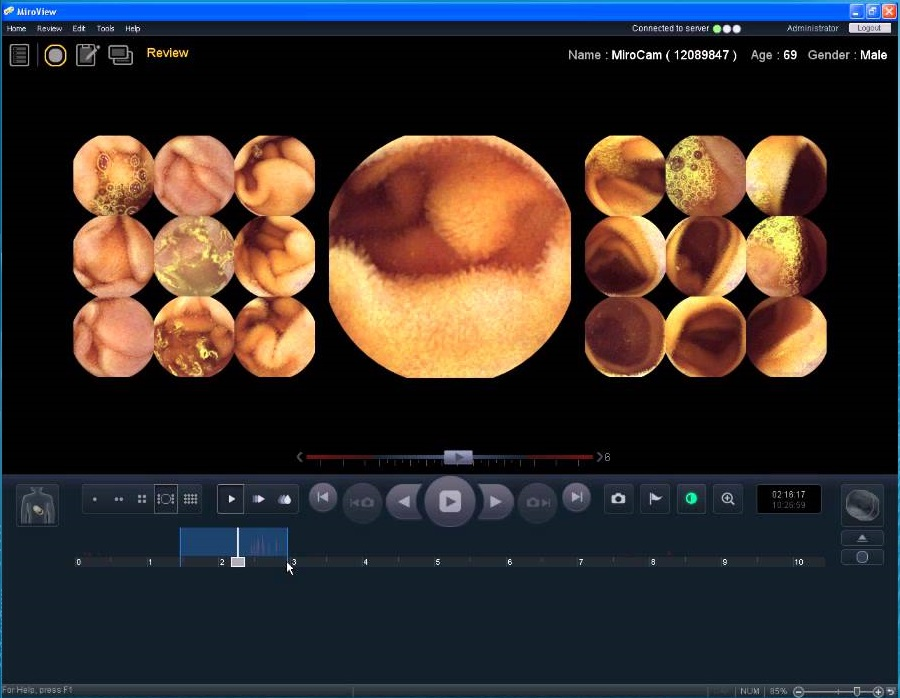
\includegraphics[scale=0.7]{miroview}
	\centering
	\caption{Ukázka MiroView 2.5\cite{miroview}\label{fig:miroview}}
\end{figure} 
\FloatBarrier
\clearpage
\subsection{GISentinel}
GISentinel je software vyvinutý společností Xyken ve spolupráci s Mayo Klinikou\footnote{Jedna z nejlepších klinik v USA, mimo jiné se také soustředí na výzkum. Spolupracuje i s ČR.\cite{about}}. Jejich software umí detekovat krev, polypy a vředy. Je k dispozici také na platformu Android, což umožňuje značnou mobilitu. Ukázka rozhraní je vidět na obrázku\ref{fig:gisentinel}.\cite{gisentinel}

\begin{figure}[h]
	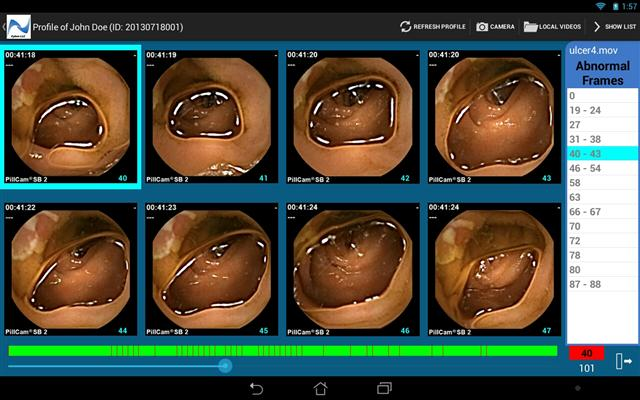
\includegraphics[scale=0.9]{gisentinel}
	\centering
	\caption{Ukázka GISentinel\cite{gisentinel}\label{fig:gisentinel}}
\end{figure}
\FloatBarrier
\begin{comment}
\section{Specifikace biomedicínských dat}
Data z kamer jsou získána, jako sled obrázků. Každý výrobce má svůj specifický vetšinou uzavřený formát. Ve všech případech se ale jedná o RGB data, která zaznamenává přímo kamera.
\end{comment}